\documentclass[xcolor=table]{beamer}
\usepackage[utf8]{inputenc}
\usepackage{default}
\usepackage{xspace,setspace}
\usepackage{amsmath,amsthm,amssymb}
\usepackage{ellipsis}
\usepackage[pdftex]{epsfig}
\usepackage{listliketab}
\usepackage[table]{xcolor}
\usepackage{booktabs}
\usepackage{amsmath}
\usepackage{amssymb}
\usepackage{eurosym}

\usepackage{pgf}
\usepackage{tikz}
\usetikzlibrary{arrows,automata}
\usetikzlibrary{graphs}
\tikzset{
     mainNode/.style =
        { circle
        , draw
        %, fill=blue!20,
        %, font=\sffamily\Large\bfseries
        }
}

\usetheme{AnnArbor}
%\usetheme{Berlin}
%\usetheme{Bergen}
%\usetheme{Antibes}
%\usetheme{Goettingen}
%\usetheme{Warsaw}
%\usetheme{Darmstadt}
%\usetheme{JuanLesPins}
%\setbeamertemplate{navigation symbols}{}
%\usecolortheme{beaver}
%\usecolortheme{rose}
%\usecolortheme{seagull}
%\usecolortheme{dove}
%\usecolortheme{seahorse}
%\usecolortheme{crane}
%\usepackage{color,colortbl}
%\usepackage{texnansi}
%\usepackage{marvosym}
%\usepackage{comment}


%\setbeamertemplate{frametitle}
%{\begin{centering}\smallskip
%   \insertframetitle\par
%   \smallskip\end{centering}}
%\setbeamertemplate{itemize item}{$\bullet$}
%\setbeamertemplate{navigation symbols}{}
%\setbeamertemplate{footline}[text line]{%
%    \hfill\strut{%
%        \scriptsize\sf\color{black!60}%
%        \quad\insertframenumber
%    }%
%    \hfill
%}

% Define some colors:

\definecolor{DarkFern}{HTML}{407428}
\definecolor{DarkCharcoal}{HTML}{4D4944}
\colorlet{Fern}{DarkFern!85!white}
\colorlet{Charcoal}{DarkCharcoal!85!white}
\colorlet{LightCharcoal}{Charcoal!50!white}
\colorlet{AlertColor}{orange!80!black}
\colorlet{DarkRed}{red!70!black}
\colorlet{DarkBlue}{olive!70!black}
\colorlet{DarkGreen}{green!70!black}
\definecolor{brickred}{RGB}{132,31,39}

% Use the colors:

%\setbeamercolor{title}{fg=Fern}
%\setbeamercolor{frametitle}{fg=Fern}
%\setbeamercolor{section title}{fg=Fern}
%\setbeamercolor{section in toc}{fg=Fern}
%\setbeamercolor{section name}{fg=Fern}
%\setbeamercolor{section in head/foot}{fg=Fern}
%\setbeamercolor{subsection title}{fg=Fern}
%\setbeamercolor{author}{fg=Fern}
%\setbeamercolor{normal text}{fg=Charcoal}
%\setbeamercolor{block title}{fg=black,bg=Fern!25!white}
%\setbeamercolor{block body}{fg=black,bg=Fern!25!white}
%\setbeamercolor{alerted text}{fg=AlertColor}
%\setbeamercolor{itemize item}{fg=Charcoal}

%\definecolor{bottomcolour}{rgb}{0.32,0.3,0.38}
%\definecolor{middlecolour}{rgb}{0.08,0.08,0.16}
\definecolor{tcsyellow}{RGB}{253,255,102}
\definecolor{tcsolive}{RGB}{77,147,191}
\definecolor{tcsolivemedium}{RGB}{147,177,210}
\definecolor{tcsolivelight}{RGB}{235,239,252}

\definecolor{skyolive}{rgb}{0.2,0.6,1}
\definecolor{darkolive}{rgb}{0.1,0.1,0.6}
\definecolor{darkred}{rgb}{1,0.2,0.1}
\definecolor{darkgreen}{rgb}{0.5,0.8,0.4}
\definecolor{Olive}{rgb}{0,0.3,0}
\definecolor{seagreen}{rgb}{0.3,0.9,0.6}
\definecolor{olive}{cmyk}{0.8,0.1,0.95,0.40}
\definecolor{golden}{cmyk}{0.0,0.25,0.85,0.15}
\definecolor{darkgolden}{cmyk}{0.0,0.27,0.94,0.07}
\definecolor{orange}{cmyk}{0.0,0.35,1.0,0.07}
\definecolor{orange2}{cmyk}{0.0,0.6,1.0, 0.0}
\definecolor{pecan}{cmyk}{0.0,0.37,0.80,0.12}
\definecolor{cadmium}{cmyk}{0.0,0.40,0.93,0.00}
\definecolor{snake}{cmyk}{0.8,0.1,0.95,0.60}
\definecolor{tcsyellow}{RGB}{253,255,102}
\definecolor{tcsolive}{RGB}{77,147,191}
\definecolor{tcsolivemedium}{RGB}{147,177,210}
\definecolor{tcsolivelight}{RGB}{235,239,252}

\definecolor{LRed}{rgb}{1,.8,.8}
\definecolor{MRed}{rgb}{1,.6,.6}
\definecolor{HRed}{rgb}{1,.2,.2}

\newtheorem{defn}{Definition}
\newtheorem{asf}{ASF Inputs}
\newtheorem{claim}{Claim}

\setbeamercolor{item projected}{bg=darkred}
\setbeamertemplate{enumerate items}[orange2]
\setbeamercolor{frametitle}{fg=white,bg=orange2}
\setbeamercolor{title}{fg=white,bg=orange2}
 
\usetheme{boxes}
\setbeamertemplate{blocks}[rounded][shadow=false]
\setbeamertemplate{itemize item}{\color{orange2}$\blacktriangleright$}
\setbeamertemplate{itemize subitem}{\color{orange2}$\blacktriangleright$}
 
\setbeamercolor{block title}{use=structure,fg=brickred,bg=white}
\setbeamercolor{block body}{use=structure,fg=black,bg=white}
 

\usefonttheme{professionalfonts}
% default | professionalfonts | serif |	structurebold | structureitalicserif |structuresmallcapsserif
%\usepackage{eulervm}

%% User defined commands
\newcommand{\vect}[1]{\ensuremath{\mathbf{#1}}}
\newcommand{\trans}[1]{\ensuremath{#1}^{\scriptscriptstyle{\textsf{T}}}}
\newcommand{\calX}{\ensuremath{{\cal X}}}
\newcommand{\calY}{\ensuremath{{\cal Y}}}
\DeclareMathOperator{\sign}{sign}
\DeclareMathOperator{\RSS}{RSS}
\DeclareMathOperator{\Var}{Var}
\DeclareMathOperator{\RSE}{RSE}

%\newtheorem{theorem}{Theorem}
\title{Classification}
\begin{document}

\maketitle

\begin{frame}[t]
  \frametitle{Classification}  
\begin{itemize}
    \item Linear regression: the response variable $y$ is quantitative.
    \item Classification: $y$ is qualitative (takes on a number of discrete values).
    \item Classification problems seem to occur more often than regression problems:
		\begin{itemize}    
    		\item spam classifiers (spam or ham)
    		\item classifying whether a bank transaction is fradulent or not
    		\item given a set of symptoms, determining which medical condition a person has
    		\item classifying whether a video is suitable or unsuitable for children
    		\item MNIST: given a handwritten digit, determine which digit it actually is
    	\end{itemize} 
  \end{itemize}
\end{frame}


\begin{frame}[t]
\frametitle{Why not Linear Regression?}
\textbf{Example 1}

Consider the following (simplified) problem: given the bank balance $x$ of an individual, determine whether they are credit worthy or not.
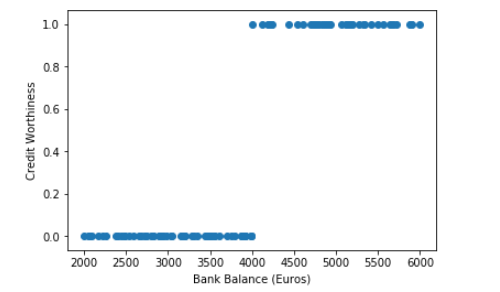
\includegraphics[scale=0.3]{bb_cw1.png}
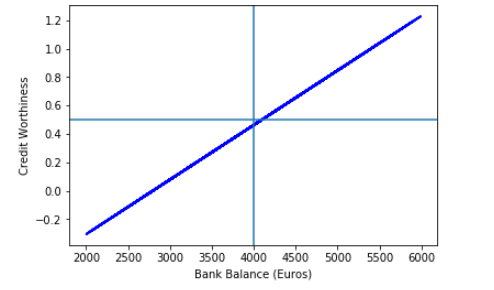
\includegraphics[scale=0.3]{lin_reg_bb_cw1.png}

\begin{itemize}
	\item Turns out that anyone with a balance of \euro 4000 or more is credit worthy
	
	\item Classification: if $y(x) \geq 0.5$, then ``credit worthy''; else ``not''
	
	\item Slope of the regression line depends on the how many data points are in each of the two buckets
\end{itemize}
\end{frame}


\begin{frame}[t]
\frametitle{Why not Linear Regression?}
\textbf{Example 1}
\begin{itemize}
	\item With more data points in the ``positive'' bucket, the slope of the regression line is less steep.
	\item The threshold predicted also changes.
\end{itemize}
 
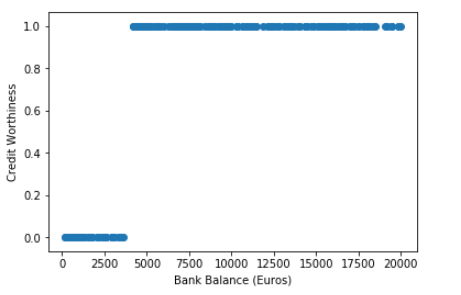
\includegraphics[scale=0.3]{bb_cw2.png}
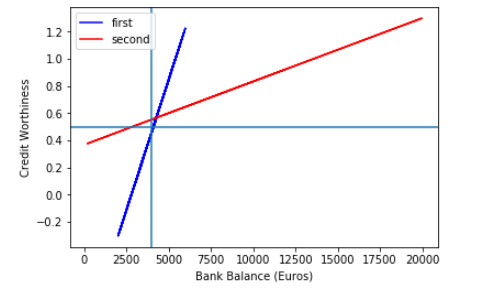
\includegraphics[scale=0.3]{lin_reg_bb_cw2.png}
\end{frame}

\begin{frame}[t]
\frametitle{Binary Classification: Logistic Regression}

\begin{itemize}
    \item  Two classes: $0$ and $1$
    
    \item Logistic regression models the probability that the response
    variable $y$ belongs to a particular class: $P(y = 1 \mid x)$
    
    \item $P(y = 1 \mid x; \theta) = g(\trans{\theta} x) = \frac{1}{1 + e^{- \trans{\theta} x}}$
    
    \item $g(z) = \frac{1}{1 + e^{- \trans{\theta} x}}$ is the sigmoid function
\end{itemize}
\end{frame}

\begin{frame}[t]
\frametitle{The Sigmoid Function}
\begin{center}
	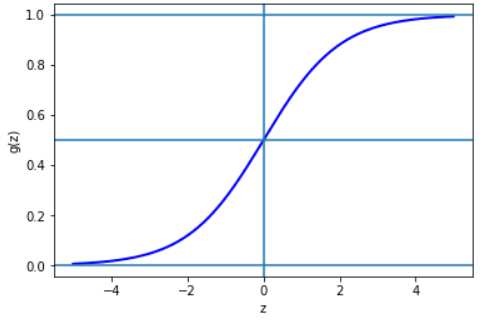
\includegraphics[scale=0.3]{sigmoid_function.png}
\end{center}

\begin{itemize}
	\item $g(z) \to 1$ as $z \to \infty$
	\item $g(z) \to 0$ as $z \to -\infty$
	\item $g'(z) = g(z) (1 - g(z))$
\end{itemize}
\end{frame}

\begin{frame}[t]
\frametitle{Logistic Regression: Learning the Model Parameters}
In logistic regression, the probabilities are modeled as follows:
\begin{equation*}
\begin{split}
P(y = 1 \mid x; \theta) & = g(\trans{\theta} x) = \frac{1}{1 + e^{- \trans{\theta} x}} \\
P(y = 0 \mid x; \theta) & = 1 - g(\trans{\theta} x) 
\end{split}
\end{equation*}

\pause

\[
	P(y \mid x; \theta) = \left( g(\trans{\theta} x) \right)^{y} \cdot 
		\left ( 1 - g(\trans{\theta} x) \right )^{1 - y}
\]

\pause

\textbf{The Likelihood Function} 

Assume that the $m$ training examples $(x^{(1)}, y^{(1)}), \ldots (x^{(m)}, y^{(m)})$ were generated \emph{independently}. 
\begin{equation*}
\begin{split}
		L(\theta; \{(x^{(i)}, y^{(i)})\}_{i = 1}^{m}) & = 
				\prod_{i = 1}^{m} P(y^{(i)} \mid x^{(i)}; \theta) \\
				& = \prod_{i = 1}^{m} \left( g(\trans{\theta} x^{(i)}) \right)^{y^{(i)}} \cdot 
						\left ( 1 - g(\trans{\theta} x^{(i)}) \right )^{(1 - y^{(i)})} \\
\end{split}
\end{equation*}
\end{frame}

\begin{frame}[t]
\frametitle{Maximizing the Likelihood $\ldots$}
$\ldots$ is equivalent to maximizing the log-likelihood:
\begin{equation*}
\begin{split}
l(\theta) & =  \log L(\theta) \\
          & = \sum_{i = 1}^{m} y^{(i)} \log g(\trans{\theta} x^{(i)}) 
          		+ (1 - y^{(i)}) \log(1 - g(\trans{\theta} x^{(i)}))
\end{split}
\end{equation*}

\begin{itemize}
	\item Use gradient ascent to maximize $l(\theta)$
	
	\item $\theta_{\text{new}} := \theta_{\text{old}} + \alpha \nabla_{\theta} l(\theta)$
	
	\item $\theta_j := \theta_j + \alpha \cdot \sum_{i = 1}^{m} \left ( y^{(i)} - 
					    g(\trans{\theta} x^{(i)}) \right ) \cdot x_j^{(i)}$
	\item Stochastic gradient ascent: $\theta_j := \theta_j + \alpha \cdot 
										(y^{(i)} - g(\trans{\theta} x^{(i)}) )\cdot x_j^{(i)}$
\end{itemize}
\end{frame}

\begin{frame}[t]
\frametitle{Classifying New Data Points}
\begin{itemize}
	\item Once $\theta$ has been estimated (using maximum likelihood, for instance),
			given $x$, $P(y = 1 \mid x) = g(\trans{\theta} \cdot x)$
	\item We could for instance classify $x$ as belonging to class~$1$ iff $g(\trans{\theta} x) \geq 0.5$
\end{itemize}
\end{frame}

\begin{frame}[t]
\frametitle{Evaluating the Performance of a Classifier}
Harder than evaluating a linear regressor.
\begin{itemize}
	\item Consider unbalanced data sets: let's say that 90\% of customers in an online store 
		are one-time customers.
	
	\item Want to determine whether a customer is a one-time customer.
	
	\item A ``dumb'' classifier that declares every customer as ``bad'' has 90\% accuracy.  
\end{itemize}
\end{frame}

\begin{frame}[t]
\frametitle{Stochastic Gradient Descent}
In batch gradient descent, the update step for the $j$th component is:
\[
    \theta_j := \theta_j  + \alpha \cdot \sum_{i = 1}^m 
        \left ( y^{(i)} - \sum_{j = 0}^n x_j^{(i)} \theta_j \right ) \cdot x_j^{(i)}.
\]

\begin{itemize}
    \item Has to scan through the entire training set for a \emph{single} update
    
    \item Costly operation if $m$ is large
    
    \pause

    \item \textbf{Stochastic Gradient Descent}: for every training instance $(x, y)$, 
    $x = \trans{(x_0, x_1, \ldots, x_n)}$, update the parameters:
    \[
         \theta_j := \theta_j  + \alpha \cdot \left ( y - \sum_{j = 0}^n x_j 
         \theta_j \right ) \cdot x_j.
    \]
\end{itemize}
\end{frame}

\begin{frame}[t]
\frametitle{Stochastic Gradient Descent: Features and Issues}
\begin{itemize}
    \item Doesn't have to look at the entire training set to make progress.

    \item Often gets close to the optimum much faster than batch gradient descent.

    \item May never converge to the optimum (can keep on oscillating between values 
    near the optimum). This problem is alleviated by choosing $\alpha$ to be very
    small.
\end{itemize}
\end{frame}

\begin{frame}[t]
\frametitle{Analytic Solution}
\[J(\theta) = 
    \frac{1}{2} \sum_{i = 1}^{m} \left (y^{(i)} - \sum_{j = 0}^{n} x^{(i)}_j \theta_j \right )^2\]  
Want to find in closed-form a value of $\theta$ that minimizes $J(\theta)$ 

\begin{itemize}
    \item Write $J(\theta)$ is matrix-vector form.
    
    \pause

    \item \textbf{Design matrix.} An $m \times (n + 1)$ matrix $X$ defined by:
    \[
        X = \left [ \begin{array}{ccc}
                        \hbox{---} & \trans{(x^{(1)})} & \hbox{---} \\
                        \hbox{---} & \trans{(x^{(2)})} & \hbox{---} \\
                        \vdots     & \vdots                   & \vdots     \\
                        \hbox{---} & \trans{(x^{(m)})} & \hbox{---} \\
                   \end{array}
            \right ]
    \]

    \pause

    \item $y = \trans{(y^{(1)}, \ldots, y^{(m)})}$
\end{itemize}
\end{frame}

\begin{frame}[t]
\frametitle{Analytic Solution $\ldots$}
\[y - X \cdot \theta =  \left [ \begin{array}{c} 
                                    y^{(1)} \\
                                    y^{(2)} \\
                                    \vdots \\
                                    y^{(m)}
                                \end{array}\right ] -
                        \left [ \begin{array}{c}
                                    \trans{(x^{(1)})} \cdot \theta \\
                                    \trans{(x^{(2)})} \cdot \theta \\
                                    \vdots                         \\
                                    \trans{(x^{(m)})} \cdot \theta \\
                                \end{array}
                       \right ]\]
Matrix-form of $J(\theta)$:
\begin{equation*}
\begin{split}
    J(\theta) & = \frac{1}{2} \sum_{i = 1}^{m} \left (y^{(i)} - \sum_{j = 0}^{n} 
                    x^{(i)}_j \theta_j \right )^2 \\
              & = \frac{1}{2} \trans{(y - X \theta)} (y - X \theta)
\end{split}
\end{equation*}
\end{frame}

\begin{frame}[t]
\frametitle{Analytic Solution $\ldots$}
Minimize $J(\theta)$ w.r.t $\theta$:
\begin{equation*}
\begin{split}
    \nabla_{\theta} J(\theta) & = \nabla_{\theta} \frac{1}{2} \trans{(y - X \theta)} (y - X \theta) \\
                              & = \text{see Andrew Ng's notes} \\
                              & = \trans{X} X \theta - \trans{X} y  
\end{split}
\end{equation*}
yielding: 
\[\boxed{\theta = (\trans{X} X)^{-1} \cdot \trans{X}y.}\] 

\pause

\begin{itemize}
    \item \textbf{Assumption:} $X$ has full column rank so that $\trans{X}X$ is invertible. \pause
    \emph{Proof.} Show that $\trans{X} X z = 0$ implies $z = 0$. 

    \pause

    \item If $X$ does not have full column rank, the usual strategy is to remove redundant columns.   
\end{itemize}
\end{frame}

\begin{frame}[t]
\frametitle{Probabilistic Interpretation}
\textbf{Assumptions}
\[
    y^{(i)} = \trans{\theta} \cdot x^{(i)} + \epsilon^{(i)},  
\]
where the error terms $\epsilon^{(i)}$
\begin{itemize}
    \item capture unmodeled effects and/or random noise

    \item are independent and identically distributed as $N(0, \sigma^2)$ 
\end{itemize}

\pause

\medskip

Given $x^{(i)}$, 
\begin{itemize}
    \item $E(y^{(i)} \mid x^{(i)}) = \trans{\theta} \cdot x^{(i)}$
    
    \pause

    \item $\Var(y^{(i)} \mid x^{(i)}) = \Var(\epsilon^{(i)}) = \sigma^{2}$
\end{itemize}

\pause

\medskip

Thus $y^{(i)} \mid x^{(i)} \thicksim N(\trans{\theta} x^{(i)}, \sigma^2)$:
\[
    p(y^{(i)} \mid x^{(i)} ; \theta ) = \frac{1}{\sqrt{2 \pi} \sigma} 
                        \exp{\left ( - \frac{(y^{(i)} - \trans{\theta} \cdot x^{(i)})^2}{2 \sigma^2}\right )}
\]
\end{frame}

\begin{frame}[t]
\frametitle{Maximum Likelihood Estimation}
\begin{itemize}
    \item Given $x = \trans{(x^{(1)}, \ldots, x^{(m)})}$ and $\theta$, what is the joint distribution of 
            the $y = \trans{(y^{(1)}, \ldots, y^{(m)})}$? 

    \pause
    
    \item Since the $\epsilon^{(i)}$s are independent: \pause 
        \[
            p(y \mid x ; \theta) = \prod_{i = 1}^{m} p(y^{(i)} \mid x^{(i)} ; \theta)
        \]

    \pause

    \item \textbf{Likelihood function.} $L(\theta) = p(y \mid x ; \theta)$ 

    \pause
        
    \[
        L(\theta) = \prod_{i = 1}^{m} \frac{1}{\sqrt{2 \pi} \sigma} 
            \exp{\left \{ - \frac{\left ( y^{(i)} - \trans{\theta} x^{(i)} \right ) ^2}{2 \sigma^2} \right \}}
    \]
    
    \pause

    \item \textbf{Principle of Maximum Likelihood.} Choose the parameters to make the data as likely 
        as possible. Choose $\theta$ to maximize $L(\theta)$.
\end{itemize}
\end{frame}

\begin{frame}[t]
\frametitle{Maximum Likelihood Estimation $\ldots$}
Maximizing $L(\theta)$ is equivalent to maximizing \emph{any} strictly increasing 
function of $L(\theta)$.

\pause

\begin{itemize}
    \item Usual to maximize the log likelihood $l(\theta) = \log L(\theta)$.

    \item $l(\theta) = m \log \frac{1}{\sqrt{2 \pi} \sigma} - 
                        \frac{1}{\sigma^2} \cdot \frac{1}{2} 
                            \sum_{i = 1}^{m}{\left ( y^{(i)} - \trans{\theta} x^{(i)} \right ) ^2}$.
    \item Maximizing $l(\theta)$ is equivalent to minimizing 
        $\frac{1}{2} \sum_{i = 1}^{m}{\left ( y^{(i)} - \trans{\theta} x^{(i)} \right ) ^2}$.
\end{itemize} 

\pause

\bigskip

\begin{block}{Summary}
Under the previous probabilistic assumptions: \textbf{least-squares regression} 
corresponds to finding the \textbf{maximum likelihood estimate} of $\theta$.
\end{block}
\end{frame}

\begin{frame}[t]
\frametitle{The Goodness of Fit}
\begin{itemize}
    \item Residual Standard Error: standard deviation of the error terms $\epsilon^{(i)}$.
    \[
        \RSE = \sqrt{\frac{1}{n - 2} \sum_{i = 1}^{m} \left ( y^{(i)} - \hat{y}^{(i)} \right )^2}
    \]

    \pause

    \item $R^2$ Statistic: 
    \[
        R^2 = 1 - \frac{ \sum_{i = 1}^{m} \left ( y^{(i)} - \hat{y}^{(i)} \right )^2}{ \sum_{i = 1}^{m} \left ( y^{(i)} - \bar{y} \right )^2}
    \]
\end{itemize}

\pause

\begin{itemize}
    \item Total sum of squares = $\sum_{i = 1}^{m} \left ( y^{(i)} - \bar{y} \right )^2$: variability 
        inherent in the response  
    
    \item Residual sum of squares = $\left ( y^{(i)} - \hat{y}^{(i)} \right )^2$: variability left 
        unexplained after performing the regression  
\end{itemize}
\end{frame}


\end{document}
